In this project it was chosen to follow an incremental design process. This was chosen because the success of this project is not well defined. The goal of picking which song to play next is a subjective decision and they can be different criteria for success.

In the incremental model the design and implementation is done one step at a time. The development is done i iterations with a new milestone for each iteration. These milestones consist of some features which we will analyse, design, implement and evaluate, documenting every step in the process. Ideas for various algorithms will be tested on multiple subjects, which we will interview for finding new possible problems or requirements, to be taken up for consideration under following iteration.

Clearly this project being very experimental, following a linear approach would require a lot of possibly not previously researches knowledge, for making descriptive analysis and design documents before even being able to test our theses on how to cope with a problem. Expected problems with the newly found solutions, would then not be handled with a new iteration.

One of the problem with the incremental model compared to the classic waterfall model is that the project can lack structure since setting milestone with clear goals is more difficult.



We will be following these steps through each iteration:

\begin{enumerate}
  \item Gathering data from users and previous iterations
  \item An brief analysis of these data, for declaring new requirements
  \item A comprehensive design phase, researching and choosing concepts in solving these requirements
  \item An effective coding period, implementing chosen the design
  \item A test of the prototype, Unit test and among users for gathering data for future iterations
\end{enumerate}

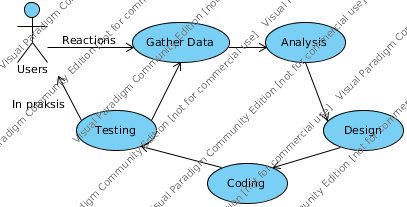
\includegraphics{Images/Developmentprocess.png}